\documentclass{standalone}

\begin{document}

\subsection[Results]{Bovine Signature}\label{bovine:bovine_result}

In the context of high-throughput data analysis, a challenge is the search for an optimal choice of variables (a \quotes{signature}) to classify groups of samples or regress trends with optimal performance and minimum dimensionality.
Usually high-throughput omics data (e.g. transcriptomics, ge-nomics, methylomics) provide datasets with few tens to hundreds of samples, and often 1000 times larger numbers of variables.
The objective of dimensionality reduction through the choice of an optimal signature is twofold: 1) the identification of relevant variables, that should separate the signal from the noise (i.e. variables not significantly associated to, or descriptive of the studied process); 2) in a practical context, it is important to establish future diagnostic criteria that can be implemented in cheap and simple toolkits, such as PCR cards or dedicated microarray chips, that usually test a small number of transcripts (ranging from tens to hundreds, at most).
The quantity of samples compared to the available features of this work, join with the final purposes of this kind of analysis, set the well-known ill-posed problem conditions for which the \textsf{DNetPRO} algorithm was thought.

Since the number of sample is drastically small no robust cross-validation procedure can be applied.
So we focused on the identification of a putative gene-signature able to discriminate between NN and NP samples, leaving the PP data as validation set.
In this case we hypothesize that PP samples will be classified more closely with NP sample rather than NN as exposed, possibly infected samples, should be more similar to positive samples, than to negative controls.

\begin{figure}[htbp]
\hspace{-1.0cm}
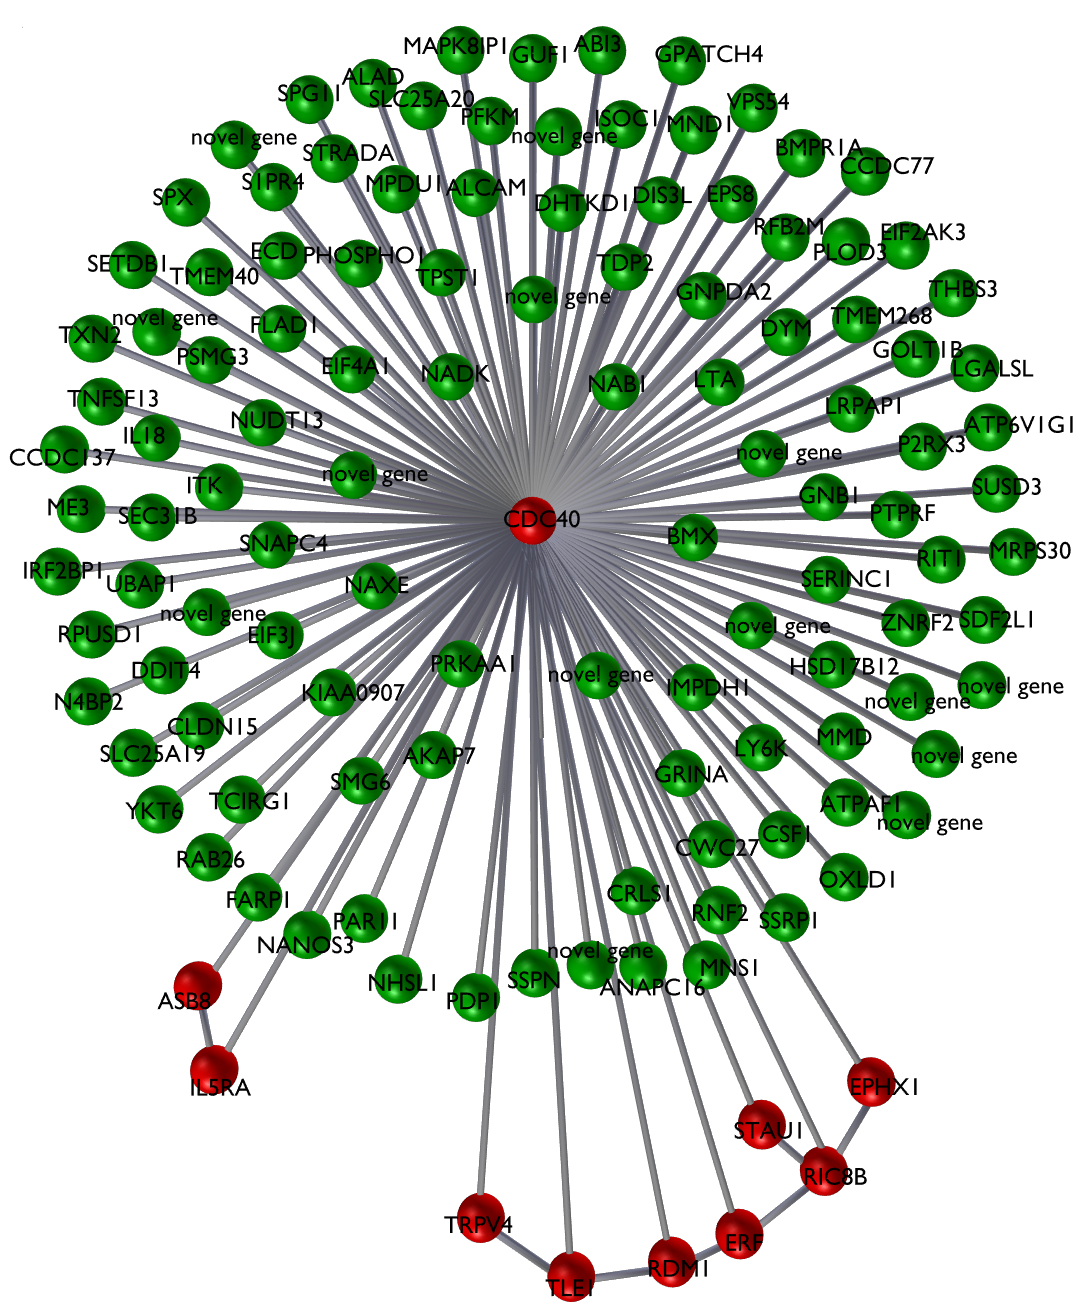
\includegraphics[width=0.4\textwidth]{Bovine_signature.png}
\qquad
\hspace{1.0cm}
\def\svgwidth{0.5\textwidth}
\input{./img/Bovine_expression_level.pdf_tex}
\caption[Caption Bovine]{(\textbf{a}) Plot of the 123-transcript network, with a details of the 10-probe signature (red nodes)\footnotemark.
(\textbf{b}) Transcript levels for the 10 genes belonging to the classification signature identified by the combinatorial discriminant analysis (CDA).
Some transcripts (EPHX1, RIC8B, IL5RA, ERF, CDC40) show a clear trend  between 5 animals serologically positive to the ELISA test for MAP (PP), 5 exposed serologically negative (NP) and 5 serologically negative unexposed control animals (NN).
}
\label{fig:bovine_signature}
\end{figure}
\footnotetext{
  The figure was generated using a custom network visualizer described in Appendix C - BlendNet.
}


Starting from the top-performing couples of transcripts, we obtained an initial signature of 123 different transcripts (Fig~\ref{fig:bovine_signature} (a), all the nodes), capable to correctly classify 4 out of the 5 NN samples (80\%) and all 5 NP samples (100\% performance).
The average performance was therefore 90\% with Matthews correlation coefficient MCC = 0.82.
Processing the 123-transcript network by removing all pendant nodes (i.e. removing all single transcripts belonging to only one best-performing couple) we obtained a final signature with 10 transcripts with a 100\% performance classifying all NN and NP samples (Fig~\ref{fig:bovine_signature} (a), only red nodes).
As it can be seen, many nodes are directly connected to the central node (belonging to the 10-transcript signature), while only the 10 transcripts of the signature are also connected between each other.

Principal Component Analysis of the 10-transcript signature showed that in many cases there was a progressive increase or decrease in the transcript levels when passing from a healthy (NN) sample to a positive (PP) sample, passing through the infected (NP) sample class.
Fig~\ref{fig:bovine_signature} (b) shows the expression levels of the transcripts belonging to the signature for all samples.

To further validate the goodness of the signature, we generated 10000 different signatures with 10 randomly chosen transcripts, and then applied a Leave-One-Out cross validation procedure to classify all 15 samples with these signatures.
Comparing the performance of the random signatures with the true 10-transcript signature, only 50 of these signatures (corresponding to 0.5\% of the random signature distribution) produced better performance than our signature in terms of classification performance, confirming its high significance.

We even characterized the possible biological role of the signature genes, among the significantly differentially expressed genes, the cell division cycle 40 gene (CDC40) showed the smallest fold change between classes.
However in the identified signature the CDC40 gene is the most central node associated with the health status of the animals related to JD.
CDC40 was also under expressed in the NP and PP groups, compared with the NN group and it has been shown to be involved in clathrin medated endcytosis from a biological point-of-view.
Clathrin is the best characterized coat protein involved in the endocytosis process, specifically in receptor-mediated-internalization.
\emph{Mycobacterium paratuberculosis} enters the host macrophages, its primary target cell, and manages to survive within their phagosome.
It is possible that the under-expression of CDC40 in infected and sick animals compared to unexposed animals may be associate with down regulation of macrophage genes post mycobacterial invasion, facilitating the survival of the pathogen with the host target cell.

Interestingly within the set of 10 discriminating transcripts, in addition to CDC40, others show links with immune response mechanisms, these include IL5RA, ERF and TRPV4.
These genes potentially have functions related to the biology of progression of JD.
Also for the other genes of the final 10-transcript signature a possible biological interpretation related to JD was given (see the original paper for further descriptions).

In conclusion, the \textsf{DNetPRO} algorithm identified a set of 10 genes, the expression levels of which could discriminate between the exposed and sero-converted animals.
These finding lead the possible use of RNA expression analysis as new diagnostic test for JD.
In particular the approach may be able to identify infected animals prior to sero-conversion, prior to a positive ELISA test result.
However, further tests for specificity and validation in a larger cohort are required.


%Description of the bovine dataset with biological background.
%Application of the \textsf{DNetPRO} on the Bovine dataset with the description of the two singatures extracted.
%Discussion on biological interpretation of the genes.

% cite and describe BlendNet repo in the signature figure

\end{document}
